
\section{Espacios topológicos}
\subsection{Espacios métricos}
Sea $X$ un conjunto no vacío.
\begin{ndef}[Distancia]
  Una \textbf{distancia} en $X$ es una aplicación $X \times X \to \R$ tal que:
  \begin{enumerate}[label=D{{\arabic*}}]
    \item $d(x,y)=0 \Leftrightarrow x=y \quad \forall x,y \in X$
    \item (Simetría) $d(x,y)=d(y,x) \quad \forall x,y \in X$
    \item (Desigualdad triangular) $d(x,y) \le d(x,z)+d(z,y) \quad \forall x,y,z \in X$
  \end{enumerate}
\end{ndef}
\begin{note}
  La propiedad $d(x,y) \geq 0 \ \forall x,y \in X$ se obtiene a partir de la definición dada de distancia.
\end{note}
\begin{proof}
  $0 \stackrel{D1}{=} d(x,x) \stackrel{D3}{\leq} d(x,y)+d(y,x) \stackrel{D2}{=} d(x,y)+d(x,y)=2d(x,y) \implies \implies d(x,y) \geq 0$
\end{proof}

\begin{exmp}
  Si $d$ es distancia en $X$ y $r>0$, entonces $rd: X \times X \to \R$ tal que $(rd)(x,y) = r \cdot d(x,y)$ es una distancia en $X$.
\end{exmp}
\begin{exmp}
  Tomemos $X=\R$. Ahora definimos $d(x,y)=|x-y| \ \forall x,y \in \R$. Entonces $d$ es una distancia en $\R$.
\end{exmp}
\begin{proof}
  Para demostrarlo, veamos que se cumplen las tres condiciones necesarias de una distancia:
  \begin{enumerate}[label=D{{\arabic*}}]
    \item $d(x,y)=0 \Leftrightarrow |x-y|=0 \Leftrightarrow x=y \quad \forall x,y \in \R$
    \item $d(x,y)=|x-y|=|0-(x-y)|=|y-x|=d(y,x) \quad \forall x,y \in \R$
    \item $d(x,y)=|x-y|=|x-z+z-y| \le |x-z|+|z-y|=d(x,z)+d(z,y) \quad \forall x,y,z \in \R$
  \end{enumerate}
\end{proof}
\begin{exmp}
  Sea $X$ un conjunto no vacío. La \textbf{distancia discreta} en $X$ es la aplicación $d:X \times X \to \R$ definida por:
  \[ d(x,y)=
    \begin{cases}
      0, & \text{si } x=y \\ 1,& \text{si } x\neq y
    \end{cases}\]
\end{exmp}
\begin{proof}
  Verifiquemos que cumple las tres propiedades:
  \begin{enumerate}[label=D{{\arabic*}}]
    \item $d(x,y)=0 \Leftrightarrow x=y \ \forall x,y \in X$ por la propia definición de $d$.
    \item $d(x,y)=d(y,x) \ \forall x,y \in X$ también por la definición dada, pues sólo depende de  que $x=y$ o $x \neq y$.
    \item Queremos probar que $d(x,y) \leq d(x,z)+d(z,y)$. Luego distinguimos dos casos:
          \begin{itemize}
            \item Si $d(x,y)=0 \implies 0 \leq d(x,z)+d(z,y)$, pues los valores que toman dichas distancias sólo pueden ser 0 o 1.
            \item Si $d(x,y)=1$, entonces $x \neq y$. Queremos ver que $1 \leq d(x,z)+d(z,y)$. Esta desigualdad se cumple si $d(x,z)=1$ o $d(z,y)=1$. Si no se cumpliera alguna de estas desigualdades, entonces $d(x,z)=d(z,y)=0$ y se tiene que $x=z=y$. Por tanto $x=y!!$, lo cual es una contradicción porque habíamos supuesto  que $x \neq y$.
          \end{itemize}
  \end{enumerate}
\end{proof}

Sea $\R^n$ el conjunto definido tal que $\R^n=\{(x_1,\cdots,x_n):x_i \in \R, \ i=1,\cdots,n\}$
\begin{ndef}[Norma]
  Una \textbf{norma} en $\R^n$ es una aplicación $\|\cdot\|: \R^n \to \R$ con las siguientes propiedades:
  \begin{enumerate}[label=N{{\arabic*}}]
    \item $\|x\|=0 \Leftrightarrow x=0 \quad \forall x \in \R^n$
    \item $\|\lambda x\|=|\lambda| \cdot \|x\|\quad \forall x \in \R^n, \forall \lambda \in \R$
    \item $\|x+y\| \le \|x\|+\|y\| \quad \forall x,y \in \R^n$
  \end{enumerate}
\end{ndef}
\begin{exmp}
  Tomando el producto escalar usual de $\R^n$, con $x,y \in \R^n$ \[\langle (x_1, \cdots, x_n), (y_1,\cdots,y_n)\rangle=x_1y_1+\cdots+x_ny_n\] su norma asociada es \[\|x\|=\langle x,x\rangle^{1/2}= \left(\sum^n_{i=1}x^2_i\right)^{1/2}=(x^2_1+\cdots+x^2_n)^{1/2}\]
  a la que llamamos \textbf{norma euclídea} y denotaremos $\|\cdot\|$ o $\|\cdot\|_2$. Otras normas en $\R^n$ que no proceden del producto escalar son la \textbf{norma 1} $\|x\|_1=|x_1|+\cdots+|x_n|$ o la \textbf{norma infinito} $\|x\|_\infty = \max_{1 \leq i \leq n} \{|x_i|\}$.
\end{exmp}

\begin{nprop}
  Toda norma $\|\cdot\|$ en $\R^n$ induce una distancia $d$ tal que $d(x,y)=\|x-y\| \ \forall x,y \in \R^n$.
\end{nprop}
\begin{proof} Probemos que se cumplen la propiedades de una distancia:
  \begin{enumerate}[label=D{{\arabic*}}]
    \item $d(x,y)=0 \Leftrightarrow \|x-y\|=0 \stackrel{N1}{\Leftrightarrow} x-y=0 \Leftrightarrow x=y \quad \forall x,y \in \R^n$
    \item $d(x,y)=\|x-y\|=\|(-1)\cdot(x-y)\|\stackrel{N2}{=} |-1|\cdot\|y-x\|=\|y-x\|=d(y,x) \quad \forall x,y \in \R^n$
    \item $d(x,y)=\|x-y\|=\|x-z+z-y\| \le \|x-z\|+\|z-y\|=d(x,z)+d(z,y) \quad \forall x,y,z \in \R^n$
  \end{enumerate}
  Por tanto, $d$ es una distancia en $\R^n$.
\end{proof}
\begin{exmp}
  En el caso del ejemplo anterior, $\|\cdot\|_2$ induce a $d_2$, $\|\cdot\|_1$ a $d_1$ y $\|\cdot\|_\infty$ a $d_\infty$, tal y como indica la proposición.
\end{exmp}

\begin{properties}
  La distancia discreta en $\R^n$ no procede de ninguna norma, es decir, no existe ninguna norma en $\R^n$ cuya distancia asociada sea la discreta.
\end{properties}
\begin{proof}
  Sea $d$ una distancia que procede de una norma $\|\cdot\|$ en $\R^n$. Tomamos $x=0$, $y\neq0$. Como $y \neq 0 \implies \|y\| \neq 0$. Ahora, tomemos $\lambda\in\R$ y vemos que $d(x,\lambda y) = \|\lambda y\| = |\lambda|\cdot\|y\|\neq 0$.
  Si $|\lambda| > \frac{1}{\|y\|}$, entonces $d(x,\lambda y) = |\lambda| \cdot \|y\| > \frac{1}{\|y\|} \cdot \|y\|=1$. Luego $d(x,\lambda y) > 1$. Por tanto, $d$ no puede ser la distancia discreta, ya que en la distancia discreta, dos puntos están a lo sumo a distancia 1.
\end{proof}
Con esto queda probado que si una distancia $d$ en $\R^n$ procede de una norma, existen puntos a distancia arbitrariamente grande.

\begin{ndef}
  Un \textbf{espacio métrico} es un par $(X,d)$ formado por un conjunto no vacío $X$ y una distancia $d$ en $X$.
\end{ndef}
\begin{ndef}
  Diremos que un espacio métrico $(X,d)$ es \textbf{acotado} si existe $M>0$ tal que $d(x,y)\leq M \ \forall x,y \in X$.
\end{ndef}
\begin{exmp}
  Un espacio métrico cuya distancia asociada es la discreta es un espacio métrico acotado, mientras que un espacio métrico sobre $\R^n$ y una distancia inducida de una norma, es un espacio métrico no acotado.
\end{exmp}

\begin{ndef}[Bolas en un espacio métrico]
  Sea $(X,d)$ un espacio métrico, con $a \in X$,
  \begin{enumerate}
    \item La \textbf{bola abierta} de centro $a$ y radio $r$ es el conjunto $B(a,r)= \{x \in X : d(x,a) < r\}$.
    \item La \textbf{bola cerrada} de centro $a$ y radio $r$ es el conjunto $\overline{B}(a,r)= \{x \in X : d(  x,a) \leq r\}$.
    \item La \textbf{esfera} de centro $a$ y radio $r$ es el conjunto $S(a,r)= \{x \in X : d(  x,a) = r\}$.
  \end{enumerate}
\end{ndef}
\begin{note}
    Si $A,B \subset X$, $A\setminus B = \{a \in A / a \not \in B\}$. Luego $S(a,r) = \overline{B}(a,r) \setminus B(a,r)$.
\end{note}
\begin{exmp}
  Sea $(X,d)$ con la distancia discreta,
  \[ d(x,y)=
    \begin{cases}
      0, & \text{si } x=y \\ 1,& \text{si } x\neq y
    \end{cases}\]
    Entonces, la bola abierta es:
    \[ B(x,r)=
    \begin{cases}
      \{x\}, & \text{si } r \leq 1 \\ X,& \text{si } r > 1
    \end{cases}\]
    La bola cerrada:
    \[ \overline{B}(x,r)=
    \begin{cases}
      \{x\}, & \text{si } r < 1 \\ X,& \text{si } r \geq 1
    \end{cases}\]
    Y la esfera,
    \[ S(x,r)=
    \begin{cases}
      X \setminus \{x\}, & \text{si } r = 1 \\ \varnothing,& \text{si } r \neq 1
    \end{cases}\]
\end{exmp}

\begin{exmp}
  En $\R^2$ con la distancia Euclídea, las bolas descritas serían de la siguiente forma en el espacio métrico $(\R^2,d_2)$:
  \begin{center}
  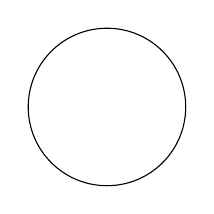
\begin{tikzpicture}
    \draw (2,2) circle (1cm);
  \end{tikzpicture}
\end{center}
\end{exmp}

\begin{properties} Estas son algunas propiedades de las bolas:
  \begin{enumerate}
    \item $a \in B(a,r),\ a \in \overline{B}(a,r) \quad \forall a \in X,\ \forall r>0$
    \item $B(a,r) \subset \overline{B}(a,r) \quad \forall a \in X,\ \forall r>0$
    \item Si $r \leq s$, entonces $B(a,r) \subset B(a,s)$ (también $\overline{B}(a,r) \subset \overline{B}(a,s)$) $\quad \forall a \in X$
    \item Si $0<\lambda<1$, entonces $B(a,\lambda r) \subset B(a,r) \quad \forall a \in X,\ \forall r>0$
  \end{enumerate}
\end{properties}

\begin{ndef}[Abierto]
  Sea $(X,d)$ un espacio métrico, diremos que $A \subset X$ es \textbf{abierto} en $(X,d)$ si, para todo $a \in A$, $\exists r > 0$ (que depende de $a$) tal que $B(a,r) \subset A$.
\end{ndef}
\begin{note}
    Siempre supondremos que $A = \varnothing$ es abierto, ya que la condición se cumple trivialmente, al ser un "para todo" sobre el vacío.
\end{note}
\begin{properties}
  Las bolas abiertas en un espacio métrico son conjuntos abiertos.
\end{properties}
\begin{proof}
  Sea $U=B(a,r),\ a \in X,\ r>0$. Sea $x \in B(a,r) \implies d(x,a)<r \implies s=r-d(x,a)>0$. Vamos a ver que $B(x,s) \subset B(a,r)$ usando la desigualdad triangular. Entonces tenemos que $z \in B(x,s) \implies d(x,z)<s \implies d(a,z) \leq d(a,x) + d(x,z)<d(a,x)+s=d(a,x)+(r-d(x,a))=r \implies z \in B(a,r) \implies B(x,s) \subset B(a,r)$. Queda probado que para todo punto $x \in B(a,r)$, existe $s>0$ que depende de $x$ al que $B(x,s) \subset B(a,r)$. Por tanto, $B(a,r)$ es un conjunto abierto.
\end{proof}
\begin{exmp}
  En un espacio métrico discreto, los puntos son conjuntos abiertos puesto que $B(a,r)=\{a\}$ si $r \geq 1$.
\end{exmp}
\begin{exmp}
  $X$ es un conjunto abierto, puesto que si $x \in X$ y $r>0$ es arbitrario, entonces $B(x,r) \subset X$.
\end{exmp}

\begin{ndef}
    Sea $(X,d)$ un espacio métrico. La \textbf{topología inducida} por $d$ es la familia $T_d \subset P(X) = \{\text{subconjuntos de X} \}$ formado por los conjuntos abiertos.
\end{ndef}
\begin{nprop}
  Sea $(X,d)$ un espacio métrico, y sea $T_d$ la topología inducida. Entonces:
  \begin{enumerate}
    \item $\varnothing ,X \in T_d$
    \item $\{U_i\}_{i \in I} \subset T_d \Rightarrow \bigcup_{i \in I} U_i \in T_d$
    \item $U_1, \cdots, U_k \in T \implies U_1 \cap \cdots \cap U_k \in T$
  \end{enumerate}
\end{nprop}
\begin{proof}
  Dem
\end{proof}

\begin{exmp}[La intersección de abiertos no tiene por qué ser un abierto]
  Sea $(\R,d)$ un espacio métrico de los reales con la distancia usual, fijamos $x=0,\ \forall r>0,\ (-r,+r) \in T$. Si tomamos $\cap_{r>0}(-r,r)=\{0\}$. El $\{0\}$ no es abierto porque no existe $s>0$ tal que $B(0,s)=(-s,s) \subset \{0\}$.
\end{exmp}

\begin{ndef}
  Decimos que dos distancias son \textbf{métricamente equivalentes} para un conjunto $X$ y $d,\ d'$ distancias en $X$ si existe $\alpha,\beta>0\ /\ \alpha d \leq d' \leq \beta d$.
\end{ndef}
\begin{properties}
  Dos distancias métricas equivalentes tienen los mismos conjuntos abiertos.
\end{properties}
\begin{properties}
  Con dos distancias métricamente equivalentes, las sucesiones convergentes son las mismas y tienen los mismos límites. Es decir la noción de sucesión convergente no depende de la distancia. Matemáticamente,
  $x_i \to x \Leftrightarrow \forall U \in T\ /\ x\in U,\ \exists b \in \N\ /\ x_i \in U\ \forall i \geq i_0$.
\end{properties}
\begin{exmp}
  En $\R^n$, $d_1,\ d_2$ y $d_\infty$ son distancias métricamente equivalentes.
  \begin{table}[t]
    \begin{center}
    \begin{tabular}{  c  c  c  }
    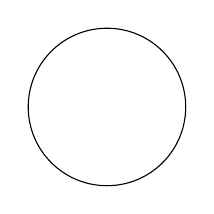
\begin{tikzpicture}
      \draw (2,2) circle (1cm);
    \end{tikzpicture}
    & 
    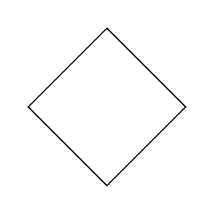
\begin{tikzpicture}
      \draw (1,0) -- (2,1) -- (1,2) -- (0,1) -- (1,0);
    \end{tikzpicture}
    &
    \begin{tikzpicture}
      \draw (0,0) -- (2,0) -- (2,2) -- (0,2) -- (0,0);
    \end{tikzpicture} \\
     $\|\cdot\|_2$ & $\|\cdot\|_1$ & $\|\cdot\|_{\infty}$ \\
    \end{tabular}
    \caption{Comparación de bolas}
    \label{tab:bolas}
    \end{center}
    \end{table} 
\end{exmp}

\begin{nprop}
  Sea $(X,d)$ un espacio métrico. Entonces todo conjunto abierto no vacío es unión de bolas abiertas.
\end{nprop}
\begin{proof}
  Sea $U \in T$. Por definición de conjunto abierto, para todo $x \in U,\ \exists r_x>0\ /\ B(x,r_x) \subset U$. Veamos que $U=\cup_{x \in U}B(x,r_x).$ \\ $B(x,r_x) \subset U\ \forall x\in U \implies \cup_{x\in U}B(x,r_x) \subset U$, quedando demostrada la primera implicación. Por otro lado, tomamos $z \in U \implies B(z,r_z) \subset U \implies z \in B(z,r_z) \subset \cup_{x \in U}B(x,r_x) \implies U \subset \cup_{x \in U}B(x,r_x)$.
\end{proof}

Ahora nos preguntamos, ¿puede ser un abierto $U \neq \varnothing $ unión de bolas cerradas? La respuesta es sí,  veámoslo: \\

Si $x \in U \ \exists r_x>0\ /\ B(x,r_x) \subset U$. Pero $\overline{B}(x, \frac{r_x}{2}) \subset B(x,r_x)$. Luego tomando $z \in \overline{B}(x,\frac{r_x}{2}) \implies d(x,z) \le \frac{r_x}{2} \le r_x \implies < \in B(x,r_x)$. Razonando como antes llegamos a que $U = \bigcup_{x \in U} \overline{B}(x,\frac{r_x}{2})$.

\begin{ndef}[Cerrado]
  Sea $(X,d)$ un espacio métrico. Diremos que $F \subset X$ es cerrado si su complementario $F^c$, $X \setminus F$, es un conjunto abierto. \[ X\setminus F = \{x \in X\ /\ x \notin F\}\]
\end{ndef}
\begin{properties}
 Los conjuntos cerrados cumplen las siguientes propiedades:
    \begin{enumerate}
    \item $\varnothing ^c=X \in T$, $X^c=\varnothing \in T\implies \varnothing ,X$ son conjuntos cerrados.
    \item Sea $\{F_i\}_{i \in I}$ una familia de conjuntos cerrados, entonces $(\cap_{i \in I}F_i)^c = \cup_{i \in I}F_i^c \in T \implies \cap_{i \in I}F_i$ es cerrado.
    \item Sea $F_1,\ldots,F_k$ una familia finita de conjuntos cerrados, entonces $(F_1 \cup \ldots \cup F_k)^c=F_1^c \cap \ldots \cap F_k^c \in T \implies F_1 \cup \ldots \cup F_k$ es un conjunto cerrado.
    \end{enumerate}
\end{properties}
  \textbf{¿Es la unión arbitraria de conjuntos cerrados, en general, cerrada?} La respuesta es no.
  \begin{exmp}
    Un ejemplo sería $(-1,1)=\cup_{n \in \N}[-1+\frac{1}{n},1-\frac{1}{n}]$, donde la primera parte de la igualdad no es cerrada mientras que la segunda sería una familia de cerrados $(\overline{B}(0,1-\frac{1}{n}))$.
  \end{exmp}
  \begin{ndef}
      A la familia de conjuntos cerrados de un espacio métrico la denotamos por $C_{T_d}$.
  \end{ndef}

\begin{properties}
  Las bolas cerradas en un espacio métrico son conjuntos cerrados.
\end{properties}
\begin{proof}
  Sean $x \in X$, $r>0$. Para que $\overline{B}(x,r)$ sea un conjunto cerrado, vamos a comprobar que $X \setminus \overline{B}(x,r)$ es un conjunto abierto. $z \in \overline{B}(x,r) \Leftrightarrow d(x,z) \leq r$. Ahora como $z \in X \setminus \overline{B}(x,r) \Leftrightarrow z \notin  \overline{B}(x,r) \Leftrightarrow d(z,x)>r$. Entonces $X \setminus \overline{B}(x,r) = \{z \in X\ /\ d(z,x)>r\}$. Veamos que es abierto. Tomamos $y \in X \setminus \overline{B}(x,r) \implies d(x,y)>r$. Definimos $s=d(x,y)-r>0$ y veamos que $B(y,s) \subset X \setminus \overline{B}(x,r)$. Sea $z \in B(y,s) \implies d(z,y)<s=d(x,y)-r$. Queremos ver que $z \in X \setminus \overline{B}(x,r)$. Es decir, que $d(x,z)>r$. Finalmente, \[d(x,y) \le d(x,z) + d(z,y) < d(x,z) + s= d(x,z)+d(x,y)-r \implies d(x,z)>r\]
\end{proof}

\begin{properties}
  Sea $(X,d)$ un espacio métrico y $x,y \in X$ con $x \neq y$. Existen entonces dos conjuntos abiertos $U_x,\ U_y$ tales que $x \in U_x,\ y \in U_y$ y $U_x \cap U_y \neq \varnothing $.
\end{properties}
\begin{ndef}[Hausdorff]
  Dicha propiedad se conoce como la propiedad $T_2$ o \textit{Hausdorff}.
\end{ndef}
\begin{proof}
  Sean $x \neq y$. Entonces $r=d(x,y)>0$ y tomamos $U_x = B(x,\frac{r}{2}),\ U_y=B(y,\frac{r}{2})$. Veamos que $U_x \cap U_y=\varnothing $. Para comprobar que $U_x \cap U_y=\varnothing $, razonemos por contradicción suponiendo que $U_x \cap U_y \neq \varnothing $. Tomemos $z \in U_x \cap U_y$. Entonces $d(x,y) \le  d(x,z) + d(z,y) < \frac{r}{2} + \frac{r}{2} = r$, ya que $z \in U_x=B(x,\frac{r}{2}) \implies d(x,z)<\frac{r}{2}$ y $z \in U_y=B(y,\frac{r}{2}) \implies d(z,y)<\frac{r}{2}$. Esta contradicción demuestra que no existe $z \in U_x \cap U_y$. Por tanto, $U_x \cap U_y = \varnothing $.
\end{proof}

\subsection{Topologías. Aspectos generales y propiedades}
\begin{ndef}[Topología]
  Sea $X$ un conjunto no vacío. Una \textbf{topología} en $X$ es una familia de $T$ de subconjuntos de $X$ ($T \subset P(x)$) que verifica:
  \begin{enumerate}
    \item $\varnothing ,X \in T$
    \item $\{U_i\}_{i \in I} \subset T \implies \bigcup_{i \in I} U_i \in T$
    \item $U_1,\ldots,U_k \in T \implies U_1 \cap \ldots \cap U_k \in T$
  \end{enumerate}
\end{ndef}
\begin{note}
    A los elementos de $T$ los llamamos \textbf{conjuntos abiertos de la topología} $T$.
\end{note}
\begin{ndef}[Espacio topológico]
  Un \textbf{espacio topológico} $(X,T)$ es un conjunto $X$ no vacío en una topología $T$ en $X$.
\end{ndef}
\begin{exmp}
  Sea $(X,d)$ un espacio métrico, $T=\{U \subset  X / \forall x \in U, \exists r>0$ tal que $B(x,r) \in U\} \cup \{\varnothing \}$. $T_d$ es una topología en $X$ y la llamaremos la topología asociada a la distancia $d$.
\end{exmp}
Sin embargo, ahora nos surge un problema. Dado un espacio topológico $(X,T)$, ¿existe una distancia en $d$ tal que $T_d=T$? Pues en general no.
\begin{ndef}[Espacio topológico metrizable]
  Un espacio topológico es \textbf{metrizable} si existe una distancia $d$ en $X$ tal que $T_d=T$.
\end{ndef}
\begin{exmp}
  Sea $X \neq \varnothing $, $T_t=\{\varnothing ,X\}$ la \textbf{topología trivial}, que es la topología con la menor cantidad posible de conjuntos. Si $T$ es otra topología en $X$, entonces $T_t \in T$ (ya que $U \in T_t \implies U \in T$).
\end{exmp}
\begin{exmp}
  Sea $X \neq \varnothing $, $T_D = P(X) = \{U / U \in X\}$ la \textbf{topología discreta}. Es la topología con el mayor número posible de conjuntos. Si $T$ es una topología cualquiera en $X$, entonces $T \subset P(X)=T_D$.
\end{exmp}
\begin{properties}
  Sea $X \neq \varnothing $, $d$ la distancia discreta y $T_D$ la topología discreta en $X$. Entonces $T_d=T_D$ y por tanto $(X,T_D)$ es metrizable.
\end{properties}
\begin{proof}
  Queremos ver que $T_d = T_D$. La inclusión $T_d \subset T_D$ se sigue de que toda topología de $X$ está contenida en $T_D$. Falta ver que $T_D \in T_d$. Sea $U \in T_D$. Si $U=\varnothing \implies U \in T_d$ porque $T_d$ es topología si $U \neq \varnothing $. \[U = \bigcup_{x \in U} \{x\} = \bigcup_{x \in U} B(x,\frac{1}{2}) \in T_d \]
\end{proof}
¿Cuándo coinciden $T_t$ y $T_D$? Solo si $X=\{p\}$.\\
¿Cuántas topologías hay en un conjunto con un elemento? $T=\{\varnothing ,X\}$

\begin{exmp}
  Sea $X \neq \varnothing $. Entonces llamaremos \textbf{topología de los complementos finitos} o topología cofinita a $T_{CF}=\{U \in X\ /\ U^c$ es finito $\} \cup \{\varnothing \}$.
\end{exmp}
\begin{proof}
  Veamos que cumple las tres propiedades de una topología:
  \begin{enumerate}
    \item $\varnothing \in T_{CF}$, $X^c = \varnothing $ (0 elementos) $\implies X \in T_{CF}$
    \item $\{U_i\}_{i \in I} \subset T_{CF}$. Si $U_i = \varnothing \ \forall i \in I \implies \bigcup_{i \in I} U_i = \varnothing \in T_{CF}$. Supongamos que $\exists i_0 \in I\ /\ U_{i_0} \neq \varnothing \implies U^c_{i_0}$ es finito. Entonces \[U_{i_0} \subset \bigcup_{i \in I} U_i \implies \left(\bigcup_{i \in I} U_i \right )^c \subset U_{i_0}^c \implies \left( \bigcup_{i \in I} U_i \right) \in T_{CF} \] El cual es finito por ser subconjunto de un conjunto finito.
    \item $U_1,\ldots,U_k \in T_{CF} \implies U_1 \cap\ldots\cap U_k \in T_{CF}$. Si algún $U_{i_0} = \varnothing \implies U_1 \cap \ldots \cap U_{i_0} \cap \ldots \cap U_k = \varnothing \in T_{CF}$. Si ningún $U_i \neq \varnothing \ \forall i \in I \implies (U_1 \cap \ldots \cap U_k)^c = U_1^c \cup \ldots \cup U_k^c \in  T_{CF}$ (la unión de conjuntos finitos es finito).
  \end{enumerate}
\end{proof}

Si $X$ es finito, $T_{CF}$ coincide con la topología discreta $T_D$, pues al ser $X$ finito, cualquier complementario es abierto en la topología por lo que $T_{CF} = P(X) = T_D$. \\

Si $X$ es infinito, $(X,T_{CF})$ no es metrizable, ya que no existe una distancia $d$ en $X$ tal que $T_d=T_{CF}$.
\begin{proof}
  Si $(Y,d)$ es un espacio métrico y $x \neq y$, $x,y \in Y \implies \exists U_x \in T_d, U_y \in T_d\ /\ U_x \cap U_y = \varnothing $. En un espacio métrico siempre podemos encontrar dos abiertos $U,V \in T_d$ tales que $U \cap V = \varnothing $.
\end{proof}

\begin{ndef}
  Un espacio topológico $(X,T)$ es \textbf{Hausdorff} (o verifica el axioma de separabilidad $T_2$ o en $T_2$) cuando, para todo par de puntos $x,y \in X$, con $x \neq y$, existen dos abiertos $U_x,U_y \in T$ tales que:
  \begin{enumerate}
    \item $x \in U_x, y \in U_y$
    \item $U_x \cap U_y = \varnothing $
  \end{enumerate}
\end{ndef}

\begin{exmp}
  Si $(X,d)$ es un espacio métrico, entonces $(X,T_d)$ es Hausdorff.
\end{exmp}
\begin{exmp}
  Si $X$ es infinito, $(X,T_{CF})$ no es Hausdorff.
\end{exmp}
\begin{exmp}
  Si $(X,T_D)$ es un espacio discreto, entonces es Hausdorff: si $x \neq y$, $U_x=\{x\}, U_y=\{y\} \in T_D$. Como $x \neq y \implies \{x\} \cap \{y\} = \varnothing \implies U_x \cap U_y = \varnothing $.
  Otra forma de ver que $(X,T_D)$ es Hausdorff es tener en cuenta que $(X,T_D)$ es metrizable. Si $d$ es la distancia discreta en $X$, entonces$T_d=P(X)=T_D$.
\end{exmp}

\begin{exmp}
  Sea $X \neq 0$. Supongamos que $X$ es, al menos, numerable. La \textbf{topología de los complementos numerables} es $T_{CN}=\{U \subset X / U^c$ es numerable$\} \cup \{\varnothing \}$.
\end{exmp}
Si $X$ es numerable, entonces $T_{CN}=T_D$ (Si $U \subset  X$ es cualquier conjunto, $U^c \subset X$. Como $X$ es numerable y $U^c \subset X / U^c$ también es numerable $\implies U \in T_{CN} \implies T_{CN} = T_D$).

Si $X$ es infinito, ¿es $(X, T_{CN})$ metrizable?
\begin{enumerate}
  \item Si $X$ es numerable $\implies T_{CN} = T_D \implies (X,T_{CN})$ es metrizable usando la distancia discreta.
  \item Si $X$ no es numerable $\implies (X,T_{CN})$ no es Hausdorff (Si $U,V \neq \varnothing \implies U \cap V \neq \varnothing $).
\end{enumerate}

\begin{ndef}
  Sean $T_1,T_2$ topologías en $X$. Diremos que $T_1$ es \textbf{más fina} que $T_2$ si $T_2 \subset T_1$. También diremos que $T_2$ es \textbf{más gruesa} que $T_1$.
\end{ndef}

\begin{ndef}
  Sea $(X,T)$ un espacio topológico. Diremos que $F \subset X$ es \textbf{cerrado} si $F^c$ es abierto.
\end{ndef}
\begin{note}
    A la familia de todos los conjuntos cerrados de $(X,T)$ la llamaremos $C_T$.
\end{note}

\begin{properties}
  Sea $(X,T)$ un espacio topológico. Entonces:
  \begin{enumerate}
    \item $\varnothing ,X \in C_T$
    \item Si $\{F_i\}_{i \in I} \subset C_T \implies \bigcap_{i \in I} F_i \in C_T$
    \item Si $F_1,\ldots,F_k \in C_T \implies F_1 \cup \cdots \cup F_k \in C_T$
  \end{enumerate}
\end{properties}
\begin{proof}
  La demostración es idéntica a la dada para espacios métricos.
\end{proof}
\begin{note}
  Si tenemos un conjunto $X$ y una familia $C \subset P(X)$ que cumple
  \begin{enumerate}
    \item $\varnothing ,X \in C$
    \item Si $\{F_i\}_{i \in I} \subset C \implies \bigcap_{i \in I} F_i \in C$
    \item Si $F_1,\ldots,F_k \in C \implies F_1 \cup \cdots \cup F_k \in C$
  \end{enumerate}
  entonces existe una única topología $T$ en $X$ tal que $G=C$.
\end{note}
\begin{proof}
  Definimos $T=\{F^c / {F \in C}\}$. Como $C \subset P(X)$ verifica las tres propiedades, pasando al complementario, $T$ verifica las propiedades de los abiertos (habría que mostrarlo).
\end{proof}
\begin{exmp}
  Estos son algunos ejemplos:
  \begin{enumerate}
    \item $(X,T_{CF}) \quad C_{T_{CF}}=\{F \subset X / F$ es finito $\} \cup \{X\}$.
    \item $(X,T_D) \quad C_{T_D}= P(X)=T_D$.
    \item $(X,T_t) \quad C_{T_t}= \{\varnothing ,X\}=T_t$.
    \item Sea $(X,d)$ un espacio métrico, todos los puntos son conjuntos cerrados.
  \end{enumerate}
\end{exmp}

\begin{properties}
  En un espacio topológico Hausdorff todo punto es cerrado.
\end{properties}
\begin{proof}
  Sea $x \in X$. $\{x_0\} \in C_T \Leftrightarrow X \setminus \{x_0\}$ es abierto. Sea $y \in X \setminus \{x_0\} \implies y \neq x_0 \implies U_y,U_{x_0}^y = \varnothing \implies x_0 \not\in U_y \implies U_y \subset X \setminus \{x_0\}$. $X \setminus \{x_0\} = \bigcup_{y \neq x_0} U_y \in T \implies \{x_0\} \in C_T$.
\end{proof}
\begin{exmp}
  $X$ infinito con $(X,T_{CF})$ \textbf{no} es Hausdorff. Los puntos son conjuntos cerrados.
\end{exmp}

\subsection{Bases de topología}
\begin{ndef}[Base]
  Sea $(X,T)$ un espacio topológico, una \textbf{base} de la topología $T$ es una familia $B \subset T$ (los elementos de $\mathcal{B}$ son conjuntos abiertos) con la propiedad de que todo conjunto abierto puede expresarse como unión de elementos de $\mathcal{B}$.
  \begin{itemize}
    \item $\forall U \in T,\ \exists \{B_i\}_{i \in I} \subset \mathcal{B}\ /\ U=\bigcup_{i \in I} B_i$
    \item $\mathcal{B} \subset T$
  \end{itemize}
\end{ndef}
\begin{exmp}
  Varios ejemplos de bases serían:
  \begin{enumerate}
    \item Sea $(X,d)$ un espacio métrico. $\mathcal{B}=\{B(x,r)\ /\ x \in X, r>0\}$ es una base de $T_d$.
    \item MAS EJEMPLOS
  \end{enumerate}
\end{exmp}

\begin{properties}
  Sea $(X,T)$ un espacio topológico, $\mathcal{B}$ base de $T$. Entonces:
  \begin{enumerate}
    \item $\forall x \in X, \exists B \in \mathcal{B}$ tal que $x \in B$.
    \item $\forall B_1,B_2 \in \mathcal{B},\ \forall x \in B_1 \cap B_2,\ \exists B_3 \in \mathcal{B}\ /\ x \in B_3 \subset B_1 \cap B_2$.
  \end{enumerate}
\end{properties}

\begin{nth}
  Sea $X$ un conjunto, $\mathcal{B} \subset P(X)$ una familia de subconjuntos de $X$ tal que
  \begin{enumerate}
    \item $\forall x \in X$, $\exists B \in \mathcal{B}$ tal que $x \in B$.
    \item $\forall B_1,B_2 \in \mathcal{B}$, $\forall x \in B_1 \cap B_2$, $\exists B_3 \in \mathcal{B}\ /\ x \in B_3 \subset B_1 \cap B_2$.
  \end{enumerate}
  Entonces existe en $X$ una única topología $T$ tal que $\mathcal{B}$ es una base de $T$.
\end{nth}
\begin{proof}
  Definimos $T=\{U \subset T / \forall x \in U, \exists B \in \mathcal{B}$ con $ x \in B \subset U\} \cup \{\varnothing \}$. Entonces:
  \begin{enumerate}
    \item $\varnothing \in T$ (por definición). $X \in T$ por (1) ($\forall x \in X\ \exists B \in \mathcal{B}$ con $x \in B \subset X$).
    \item Sea $\{U_i\}_{i \in I} \subset T$. ¿$\bigcup_{i \in I} U_i \in T$? Si $\bigcup_{i \in I} U_i = \varnothing , \varnothing \in T$. Si $x \in \bigcup_{i \in I} U_i \implies \exists i_0 \in I / x \in U_{i_0}$. Como $U_{i_0} \in T$, $\exists B \in \mathcal{B}$ ESTE Y OTRO PUNTO.
  \end{enumerate}
  Veamos ahora que $\mathcal{B}$ es base de $T$. Tenemos que comprobar que
  \begin{enumerate}
    \item $B \subset T$.
    \item Todo $U \in T \setminus \{\varnothing \}$ es unión de elementos de $\mathcal{B}$.
  \end{enumerate}
  Tomamos $T=\{U \subset T / \forall x \in U, \exists B \in \mathcal{B}$ con $ x \in B \subset U\} \cup \{\varnothing \}$.
  \begin{itemize}
    \item Sea $B \in \mathcal{B}$. $\forall x \in B,\ x \in B \subset B$ (tomando $B=U$) $\implies \mathcal{B} \subset T$.
    \item Sea $U \in T,\ U \neq \varnothing $. Sea $x \in U \implies \exists B_x \in \mathcal{B}x \in U \implies \exists B_x \in \mathcal{B}\ /\ x \in B_x \subset U \implies U = \bigcup_{x \in U} B_x \implies U$ es unión de elementos de $\mathcal{B}$.
  \end{itemize}
  Veamos por último la unicidad de $T$. Sea $T'$ otra topología en $X$ tal que $\mathcal{B}$ es base de $T'$. Veamo que $T=T'$. \[T \subset T' \implies \exists \{B_i\}_{i \in I} \subset \mathcal{B}\ /\ U = \bigcup_{i \in I} B_i \implies U = \bigcup_{i \in I} B_i \in T' \]
  $T \subset T'$ se demuestra igual (para probar $T \subset T'$ solo hemos usado que $\mathcal{B}$ es base de $T,T'$).
\end{proof}
\begin{nprop}
  Sea $X$ un conjunto, $T_1,T_2$ dos topologías en $X$. Supongamos que $\mathcal{B}$ es base de $T_1$ y $T_2$. Entonces $T_1 = T_2$.
\end{nprop}
\begin{exmp}
  Topología de \textbf{Sorgenfrey} o del \textbf{límite inferior} $(\R,T_S)$, cuya base es $\mathcal{B}=\{[a,b)\ /\ a,b \in \R, a<b\} $.
\end{exmp}
\begin{exmp}
    Topología de \textbf{Kuratowski} o \textbf{K-Topología} $(\R, T_K)$. Dado $K = \{\frac{1}{n} : n \in \N\}$, $\mathcal{B} = \{(a,b) \setminus K :\ a,b \in \R,\ a<b\} \cup \{(a,b) :\ a<b\} \cup \{ \varnothing \}$.
\end{exmp}
Como podemos ver, tenemos otras topologías en $\R$ a parte de la usual. Para compararlas, daremos el siguiente criterio:
\begin{properties}
    Sea $X \neq \varnothing$, y sean $\mathcal{B}, \mathcal{B}'$ bases de las topologías $T,T'$ respectivamente, entonces son equivalentes:
    \begin{enumerate}
        \item $T \subset T'$.
        \item $\forall B \in \mathcal{B},\ \forall x \in X,\ \exists B' \in \mathcal{B}'$ tal que $x \in B' \subset B$.
    \end{enumerate}
\end{properties}
\begin{proof}
    Dem.
\end{proof}
\begin{ncor}
  Sean $\mathcal{B}, \mathcal{B}'$ bases de $T,T'$. Son equivalentes:
  \begin{enumerate}
    \item $T=T'$.
    \item \begin{itemize}
            \item $\forall B \in \mathcal{B}, \forall x \in B, \exists B' \in \mathcal{B}' / x \in B' \subset B \quad (T \subset T')$.
            \item $\forall B' \in \mathcal{B}', \forall x \in B', \exists B \in \mathcal{B} / x \in B \subset B' \quad (T' \subset T)$.
          \end{itemize}
  \end{enumerate}
\end{ncor}
\begin{properties}
    La topología usual es más gruesa que la topología de Kuratowski y la de Sorgenfrey, es decir, $T_u \subset T_S,\ T_u \subset T_K$.
\end{properties}
\begin{proof}
    Dem
\end{proof}
\begin{properties}
  La topología usual es distinta de la topología de Sorgenfrey y de la topología de Kuratowski, es decir, $T_u \neq T_S$, $T_u \neq T_K$.
\end{properties}
\begin{proof}
  Como $T_u \subset T_S$, buscamos $u \in T_S \setminus T_u$ tal que $u = [0,1) \in \mathcal{B} \subset T_S$. Veamos que $u \not\in T_u$. Supongamos que $u \in T_u \implies \exists \{B_i\}_{i \in J} \subset \mathcal{B}_u / 0 \in u = \bigcup_{i \in I}B_i \implies \exists i_0 \in I / 0 \in B_{i_0} \subset  \bigcup_{i \in I} B_i = u$. Luego $B_{i_0} = (a,b),\ a<b$. Entonces $0 \in (a,b) \subset [0,1)$, ya que $a<0$. Por último, tomamos $z \in (a,0) \implies z \in (a,b)$ y $z \not\in [0,1) \implies (a,b) \not\subset [0,1)!!$. Esto es una contradicción, pues suponíamos que $u \in T_u$. Luego $T_u \neq T_S$. \\
  Por otro lado, tenemos que encontrar $u \in T_K \setminus T_u$. Tomamos $u = (-1,1) \setminus K \in T_K$. Supongamos que $u \in T_u \implies \exists \{B_i\}_{i \in I} \subset \mathcal{B}_u\ /\ u = \bigcup_{i \in I}$ ACABAR
\end{proof}
\begin{properties}
    $T_S$ y $T_K$ no son comparables.
\end{properties}

\begin{lema}
  Si $X$ es un conjunto y $\{T_i\}_{i \in I}$ es una familia de topologías en $X$. Entonces \[T=\bigcap_{i \in I} T_i = \{U \subset X\ /\ U \in T_i \forall i \in I\} \] es una topología en $X$.
\end{lema}
\begin{proof}
  demostración
\end{proof}

\begin{nprop}
  Sea $S \subset P(X)$. Existe una topología $T(S)$ (topología generada por S) en $X$ tal que $S \subset T(S)$. Además, si $T'$ es otra topología que contiene a $S$, entonces $T(S) \subset T'$. Es decir, $T(S)$ es la \textbf{topología más gruesa} que contiene a S).
\end{nprop}
\begin{proof}
  proof
  ppppp
\end{proof}
\begin{exmp}
    Sea $A \subset X$, $S = \{A\}$. Entonces $T(S) = \{\varnothing, A, X\}$.
\end{exmp}
\textbf{La unión de topologías no tiene por qué ser una topología.} Veamos un ejemplo de esto:
\begin{exmp}
    Sean $T_1,T_2$ topologías en $X$. Definimos ahora $T_1,T_2 \subset T_1 \cup T_2 = \{U \subset X :\ U \in T_1 \lor U \in T_2\}$. Entonces, tomando por ejemplo $X = \{a,b,c\}$, $T_1 = \{\varnothing, \{a\}, X\}$ y $T_2 = \{\varnothing, \{b\}, X\}$, vemos que $T_1$ y $T_2$ son topologías pero $T_1 \cup T_2 = \{\varnothing, \{a\}, \{b\}, X\}$ no lo es, pues $\{a,b\} \not \in T_1 \cup T_2$.
\end{exmp}
Sin embargo, si que podemos obtener la topología generada por la unión de topologías $T(T_1 \cup T_2)$.
\begin{ndef}
    Llamaremos $T(T_1 \cup T_2)$ a la \textbf{topología generada por $T_1$ y $T_2$}. Es la topología más gruesa que contiene a $T_1$ y $T_2$.
\end{ndef}
\begin{ndef}[Subbase]
    Sea $(X,T)$ un espacio topológico y $S \subset P(X)$. Diremos que $S$ es una \textbf{subbase de} $T$ si la familia $\{\bigcap_{i \in I} S_i :\ I\text{ finito}\}$ es una base de $T$.
\end{ndef}
\begin{obs}
    Todo abierto $U \in T$ es unión arbitraria de intersecciones finitas de elementos de $S$.
\end{obs}
\begin{nprop}
  Sea $X$ un conjunto, $S \subset P(X)$. Entonces $\bigcup_{V \in S} V = X$ si, y sólo si $S$ es una subbase de $T(S)$.
\end{nprop}
\begin{proof}
    Dem
\end{proof}
\begin{nprop}
  $S$ es subbase de $T$ si $\mathcal{B}(S) = \{\bigcap_{i \in I} s_i :\ S_i \in S,\ I \text{ finito}\}$ es una base de $T$.
\end{nprop}
\begin{proof}
    Dem
\end{proof}
\begin{lema}
  Sea $(X,T)$ un espacio topológico. Para cada $x \in X$, sea $N_x$ el conjunto de entornos de $x$. Entonces:
  \begin{enumerate}
      \item $x \in U \quad \forall U \in N_x$.
      \item Si $U_1, U_2 \in N_x$, entonces $U_1 \cap U_2 \in N_x$.
      \item Si $U \in N_x$, $U \subset V$, entonces $V \in N_x$.
      \item $\forall U \in N_x$, $\exists V \in N_x$ tal que $U \in N_y \quad \forall y \in V$.
  \end{enumerate}
\end{lema}
\begin{note}
    Recordatorio: $U \in N_x$ si $\exists A \in T$ tal que $x \in A \subset U$.
\end{note}
\begin{proof}
    Dem
\end{proof}
\begin{nth}
  Sea $X \neq \varnothing$. Consideramos una colección $\{M_x\}_{x \in X}$ con $\varnothing \neq M_x \subset P(X) \ \forall x \in X$. Supongamos que:
  \begin{enumerate}
      \item $x \in U \quad \forall U \in M_x$.
      \item Si $U_1, U_2 \in M_x$, entonces $U_1 \cap U_2 \in M_x$.
      \item Si $U \in M_x$, $U \subset V$, entonces $V \in M_x$.
      \item $\forall U \in M_x$, $\exists V \in M_x$ tal que $U \in M_y \quad \forall y \in V$.
  \end{enumerate}
  Entonces $T = \{U \subset X :\ \forall x \in U,\ \exists V \in M_x \text{ tal que } V \subset U\} \cup \{\varnothing\}$ es una topología en $X$ tal que $M_x = N_x\ \forall x \in X$. Además, $T$ es la única topología tal que $N_x = M_x\ \forall x \in X$. 
\end{nth}
\begin{proof}
    Dem
\end{proof}
\begin{lema}
  Sea $(X,T)$ un espacio topológico. Entonces $U \in T$ si, y sólo si $\forall x \in U,\ \exists V \in N_x$ tal que $V \subset U$.
\end{lema}
\begin{proof}
    Dem
\end{proof}

\subsection{Puntos adherentes, interiores y frontera de un subconjunto}
Sea $(X,T)$ un espacio topológico y sea $A \subset X$, $A \neq \varnothing$.
\begin{ndef}
    Diremos que $x \in X$ es un \textbf{punto adherente} de $A$ si $V \cap A \neq \varnothing$ para todo $V \in N_x$.
\end{ndef}
\begin{note}
Dicho de manera más coloquial, un punto es adherente a $A$ si todo entorno del punto corta a $A$.
\end{note}
\begin{ndef}
    Al conjunto de puntos adherentes de $A$ se le llama la \textbf{adherencia} o \textbf{clausura} de $A$..
\end{ndef}
\begin{ndef}
    Diremos que $x \in X$ es un \textbf{punto interior} de $A$ si existe $V \in N_x$ tal que $V \subset A$.
\end{ndef}
\begin{ndef}
    El conjunto de puntos interiores de $A$ se le llama \textbf{interior} de $A$.
\end{ndef}
\begin{ndef}
  $x \in X$ es un \textbf{punto frontera} de $A$ si $\forall U \in N_x$, se tiene $U \cap A \neq \varnothing $, $U \cap A^c \neq \varnothing $.
\end{ndef}
\begin{ndef}
  $x \in X$ es un \textbf{punto de acumulación} de $A$ si $\forall U \in N_x$, se tiene $(U\setminus \{x\}) \cap A \neq \varnothing $.
\end{ndef}
\begin{ndef}
  $x \in X$ es un \textbf{punto aislado} de $A$ si $\exists U \in N_x$, se tiene $U \cap A = \{x\} $.
\end{ndef}

Entonces para $A \subset X$, denotaremos:
\begin{itemize}
  \item $int(A)$ o $A^o$ a los puntos interiores de $A$, es decir, el interior de $A$.
  \item $cl(A)$ o $\overline{A}$ a los puntos adherentes de $A$, es decir, la clausura de $A$.
  \item $fr(A)$ o $\delta A$ a los puntos frontera de $A$, es decir, la frontera de $A$.
  \item $A'$ a los puntos de acumulación de $A$.
  \item $ais(A)$ a los puntos aislados de $A$, es decir, al conjunto de puntos aislados de $A$.
\end{itemize}

\begin{ndef}
  $x \in X$ es \textbf{punto exterior} de $A$ si $x$ es punto interior de $A^c$, es decir, $\exists U \in N_x\ /\ U \subset A^c$. El conjunto de puntos exteriores de $A$ se denota por $ext(A)$.
\end{ndef}

\begin{properties}
  Dado un conjunto $A$, se tiene que $A^o \subset A \subset \overline{A}$.
\end{properties}
\begin{proof}
  \begin{itemize}
    \item $A^o \subset A$. Sea $x \in A^o \implies \exists U \in N_x\ /\ x \exists $ ACABAR
  \end{itemize}
\end{proof}
\begin{properties}
  $A^o \in T$. Además, si $U \in T$ y $U \subset A$, entonces $U \subset A^o$, es decir, $A^o$ es el mayor conjunto abierto contenido en $A$.
\end{properties}
\begin{proof}
  $A^o \in T$. Si $A^o = \varnothing $, entonces $A^o \in T$. Si $A^o \neq \varnothing $, tomamos $x \in A^o \implies \exists U \in N_{x}\ /\ U \subset A \implies \exists V \in N_x$ con $V \subset U\ /\ U \in N_y \ \forall y \in V \implies y \in A^o \ \forall y \in V \implies V \subset A^o \implies \exists W_x \in T \ /\ x \in W_x \subset V \subset A^o \implies A^o = \bigcup_{x \in A^o} W_x \in T$. Ahora, sea $U \in T\ /\ U \subset A$. Si $x \in U$, como $U \in N_x \implies x \in A^o \implies U \subset A^o$.
\end{proof}

\begin{properties}
  $\overline{A} \in C_T =$ \{\text{conjuntos cerrados en }$(X,T)\}$. Además, si $F \in C_T$ y $A \subset F$, entonces $\overline{A} \subset F$. Es decir, la clausura de $A$ es el menor conjunto cerrado que contiene a $A$.
\end{properties}
\begin{proof}
  $\overline{A} \in C_T \Leftrightarrow X \setminus \overline{A} \in T$. Sea $x \in X \setminus \overline{A} \Leftrightarrow x \not\in \overline{A} \Leftrightarrow \exists U \in N_x\ /\ U \cap A = \varnothing \Leftrightarrow U \subset X \setminus A \Leftrightarrow x \in int(X \setminus A)$. Por tanto, $X \setminus \overline{A} = int(X \setminus A) \implies X \setminus \overline{A} \in T \implies \overline{A} \in C_T$.
\end{proof}
\begin{properties}
    Sea $A \in X$, entonces $A' \subset \overline{A}$.
\end{properties}
\begin{ncor}
  Sea $A \subset X$ se cumple que:
  \begin{enumerate}
    \item $A \in T \Leftrightarrow A=A^o$
    \item $A \in C_T \Leftrightarrow A=\overline{A}$
  \end{enumerate}
\end{ncor}
\begin{proof}
  Demostremos ambas dobles implicaciones:
  \begin{enumerate}
    \item \fbox{$\Leftarrow$} Si $A=A^o$, como $A^o \in T \implies A \in T$. \\ \fbox{$\Rightarrow$} $A \in T$. Siempre $A^o \subset A$. Además $A^o$ es el mayor conjunto abierto contenido en $A$. Luego $A \in T$, $A \subset A \implies A \subset A^o$. Por tanto $A=A^o$.
    \item \fbox{$\Leftarrow$} Si $A=\overline{A}$ ACABAR
  \end{enumerate}
\end{proof}

\begin{properties}
  De lo dicho anteriormente caben destacar las siguientes propiedades:
  \begin{enumerate}
    \item $\overline{A}=A^o \cup \delta A$, $A^o \cap \delta A = \varnothing$
    \item $\delta A = \overline{A} \cap \overline{(X \setminus A)}$, en particular, $\delta A \in C_T$.
    \item $\{A^o,\delta A, ext(A)\}$ es una partición de $X$.
  \end{enumerate}
\end{properties}

\begin{exmp}
  Sea $(\R^n, \|\cdot\|)$ un espacio normado en $\R^n$ con la distancia asociada $d(x,y)=\|x-y\|$. Entonces se tiene que la clausura de la bola abierta es igual a la bola cerrada y el interior de la bola cerrada es igual a la bola abierta. Es decir, $\overline{B(x,r)}=\overline{B}(x,r)$ y $int(\overline{B}(x,r))=B(x,r)$.
\end{exmp}
Para que la propiedad del ejemplo se cumpla, la distancia debe proceder de una norma.
\begin{exmp}
  Sea $(X,d)$ un espacio métrico donde $d$ es la distancia discreta, tal que $\#X \ge 2$. Si tomamos $x \in X$, entonces se cumple que $B(x,1)=\{x\}$ y $\overline{B}(x,1)=X$. Aquí tenemos que $\overline{B(x,1)}$ es el menor conjunto cerrado que contiene a $B(x,1)$, luego $\overline{B(x,1)} \subset \overline{B}(x,1)$. Como $T_d$ es la topología discreta, $\{x\} \in C_{T_d} \implies \overline{\{x\}} = \{x\} \implies \overline{B(x,1)}=\{x\}$. Pero $\overline{B}(x,1)=X \neq \{x\} = \overline{B(x,1)} \implies \overline{B(x,1)} \subsetneq \overline{B}(x,1)$.
\end{exmp}
\begin{properties}
  Si $(X,d)$ es un espacio métrico, $x \in X$ y $r >0$, entonces $int(\overline{B}(x,r))$ es el mayor abierto contenido en $\overline{B}$. Pero $B(x,r) \subset \overline{B}(x,r) \implies B(x,r) \subset int(\overline{B}(x,r))$.
\end{properties}

\subsection{Axiomas de separación}
\begin{ndef}[Separación]
  Diremos que un espacio topológico $(X,T)$ es $T_1$ si $\forall x,y \in X,\ x\neq y,\ \exists V_x \in N_x,\ V_y \in N_y$ tales que $x \not\in V_y,\ y \not\in V_x$.
\end{ndef}
\begin{properties}
  $(X,T)$ es $T_1 \Leftrightarrow$ todo punto de $X$ es cerrado.
\end{properties}
\begin{proof}
  \fbox{$\Rightarrow$} Supongamos que $(X,T)$ es $T_1$. Fijamos $x \in X$. Veamos que $\{x\}$ es cerrado comprobando que $X \setminus \{x\}$ es abierto. Para ello, vemos que $int(X \setminus \{x\})=X \setminus \{x\}$. Sea $y \in X \setminus \{x\} \implies y \neq x$. Como $(X,T)$ es $T_1,\ \exists V_x \in N_x,\ V_y \in N_y$ tales que $x \not\in V_y,\ y \not\in V_x$. $x \not\in V_y \implies \{x\} \cap V_y = \varnothing \implies V_y \subset X \setminus \{x\} \implies y \in int(X \setminus \{x\})$. Hemos probado que  $X \setminus \{x\} \subset int(X \setminus \{x\}) \implies X \setminus \{x\} = int(X \setminus \{x\}) \implies X \setminus \{x\} \in T \implies \{x\} \in C_T$. \\
  \fbox{$\Leftarrow$} Supongamos que todo punto de $X$ es cerrado. Veamos que $(X,T)$ es $T_1$. Para ello tomaremos $x,y \in X,\ x \neq y$. Por hipótesis, $\{x\}$ es cerrado $\implies X \setminus \{x\} \in T$. Como $y \neq x,\ y \in X \setminus \{x\}$ y $X \setminus \{x\}$ es abierto, coincide con su interior $\implies \exists V_y \in N_y$ tal que $V_y \subset X \setminus \{x\} \implies x \in V_y$. Razonando igual para $x$ encontramos $V_x \in N_x$ tal que $y \not\in  V_x$.
\end{proof}

\begin{ndef}
  Diremos que un espacio topológico $(X,T)$ es $T_2$ o \textbf{Hausdorff} si $\forall x,y \in X,\ x \neq y,\ \exists V_x \in N_x,\ V_y \in N_y$ tales que $V_x \cap V_y = \varnothing$.
\end{ndef}
\begin{note}
    Si $V_x \cap V_y = \varnothing \Rightarrow x \not \in V_y,\ y \not \in V_x$.
\end{note}
Como consecuencia, \textbf{en un espacio hausdorff todo punto es cerrado}.

\begin{exmp}
  $(\N,T_{CF})$ es $T_1$ pero no es $T_2$. Ya hemos visto en clase que $(\N,T_{CF})$ no es $T_2$. Sin embargo, dicho espacio topológico es $T_1$ porque todo punto es cerrado.
\end{exmp}

\subsection{Axiomas de numerabilidad}
\begin{ndef}
  Diremos que $(X,T)$ verifica el \textbf{el primer axioma de numerabilidad} o que es $AN-I$, si cada punto de $X$ admite una base de entornos numerable.
\end{ndef}

\begin{ndef}
  Diremos que $(X,T)$ verifica el \textbf{el segundo axioma de numerabilidad} o que es $AN-II$  , si $T$ admite una base numerable.
\end{ndef}

\begin{exmp}
  Sea $(X,T_D)$ un espacio topológico discreto. Entonces $\mathcal{B}_x=\{\{x\}\}$ es base de entornos $\implies (X,T_D)$ es $AN-I$. Si $X$ es no numerable, entonces  $(X,T_D)$ no es $AN-II$.\\

  Sea $\mathcal{B}$ una base de $T$. Si $x \in X,\ \{x\} \in T_D \implies \{x\} = \bigcup_{i \in I}B_i$ tal que $B_i \in \mathcal{B} \implies \exists B_{i_0}\ /\ x \in B_{i_0} \subset \bigcup_{i \in I} B_i = \{x\}$. ACABAR
\end{exmp}

\begin{lema}
  Si $\mathcal{B}$ es base de T. Entonces $\mathcal{B}(x) = \{B \in  \mathcal{B}\ /\ x \in B\}$ es base de entornos abiertos de $x$ para todo $x \in X$.
\end{lema}

\begin{ncor}
  Si $(X,T)$ es $AN-II$, entonces es $AN-I$.
\end{ncor}
\begin{proof}
  P
\end{proof}

\begin{ndef}[Subconjunto denso]
  Diremos que un subconjunto $D$ de un espacio topológico $(X,T)$ es denso si $\overline{D}=X$.
\end{ndef}

\begin{ndef}[Separable]
  Diremos que un espacio topológico es separable si contiene un subconjunto denso y numerable.
\end{ndef}
\begin{ndef}[Convergencia]
Sea $(X, T)$ un espacio topológico, y sea $\left\{x_{n}\right\}_{n \in \mathrm{N}} \subseteq X$ una sucesión en $X$. Diremos que $\left\{x_{n}\right\}_{n \in \mathbb{N}}$ \textbf{converge a un punto} $x_{0} \in X$ en $(X, T)$, y escribiremos $\left\{x_{n}\right\}_{n \in \N} \rightarrow x$ en $(X, T)$, si $\forall U \in N_{x},\ \exists N \in \N: x_{n} \in U\ \forall n \geq N .$
\end{ndef}

En este caso, la sucesión $\left\{x_{n}\right\}_{n \in \N}$ se dirá \textbf{convergente} en $(X, T)$. También diremos que $x_{0}$ es un \textbf{limite} de $\left\{x_{n}\right\}_{n \in \N}$ en $(X, T)$.

Una de las propiedades del límite de una sucesión en un espacio métrico es su unicidad. Ese resultado no es cierto con generalidad en la categoría de espacio topológicos, pero sí en ambiente $T_{2}$.
\begin{nth}
Sea $(X, T)$ un espacio topológico $T_{2}, y$ consideremos una sucesión $\left\{x_{n}\right\}_{n \in \N}$ convergente en $(X,T)$. Entonces $\left\{x_{n}\right\}_{n \in \N}$ tiene un único limite en $(X,T)$.
\end{nth}
\begin{proof}
Razonemos por reducción al absurdo y supongamos que $\left\{x_{n}\right\}_{n \in \N}$ tiene dos límites $y_{1}$ e $y_{2}$ en $(X,T), y_{1} \neq y_{2}$. Como $(X,T)$ es $T_{2}$, existen dos entornos $U_{1} \in N_{y_{1}}$ y $U_{2} \in N_{y_{2}}$ tales que $U_{1} \cap U_{2}=\varnothing .$

Como $\left\{x_{n}\right\}_{n \in \N} \rightarrow y_{j}$ en $(X,T)$, podemos encontrar $N_{j} \in \N$ tal que $x_{n} \in U_{j}$ para todo $n \geq N_{j}$, $j=1,2$. Por tanto, para cualquier $n \geq \max \left\{N_{1}, N_{2}\right\}$ se tendrá que $x_{n} \in U_{1} \cap U_{2}$, lo que es una contradicción.
\end{proof}

\begin{nprop}
  Sean $(X, T)$ un espacio topológico $AN-I$ y $A \subset X$ un subconjunto suyo. Entonces,
$$
x \in \bar{A} \Longleftrightarrow \exists \{x_{n} \}_{n \in \N} \subset A \text { tal que } \{x_{n} \}_{n \in \N} \rightarrow x.
$$
\end{nprop}
\begin{proof}
    Dem
\end{proof}
\newpage
\section{Aplicaciones entre espacios topológicos}
\subsection{Continuidad. Caracterizaciones de la continuidad}
\begin{ndef}[Aplicación continua]
  Sean $(X,T)$, $(Y,T')$ espacios topológicos y $f: X \to Y$ una aplicación. Diremos que $f$ es una \textbf{aplicación continua} de $(X,T)$ en $(Y,T')$ si, para todo $U' \in T'$, se tiene que $f^{-1}(U') \in T$.
\end{ndef}
\begin{note}
  Si $f: X \to Y$ es una aplicación entre dos conjuntos y $U' \subset Y$,
  \[f^{-1}(U')=\{x \in X: f(x) \in U'\}\]
  donde $f^{-1}(U')$ es la imagen inversa de $U'$ por $f$ ($f^{-1}$ no es la aplicación inversa de $f$).
\end{note}
\begin{properties}
    $f^{-1}$ tiene las siguientes propiedades:
  \begin{itemize}
      \item $f^{-1}(U' \cap V')=f^{-1}(U') \cap f^{-1}(V')$
      \item $f^{-1}(U' \cup V')=f^{-1}(U') \cup f^{-1}(V')$
      \item $f^{-1}(Y \setminus U')=X \setminus f^{-1}(U')$
      \item $f(f^{-1}(U')) \subset U'$
  \end{itemize}
\end{properties}

\begin{ndef}
  Sean $(X,T)$, $(Y,T')$ espacios topológicos, $f: X \to Y$ una aplicación y $x_0 \in X$. Diremos que $f$ es continua en $x_0$ si, para todo entorno $V \in N'_{f(x_0)} = \{$entornos de $f(x_0)$ en $(Y,T')\}$, existe $U \in N_{x_0} = \{$entornos de $x_0$ en $(X,T)\}$ tal que $f(U) \subset V$.
\end{ndef}
\begin{properties}[Caracterización de continuidad por entornos]
    Sean $(X,T)$, $(Y,T')$ espacios topológicos, $f: X \to Y$ una aplicación. Son equivalentes
    \begin{enumerate}
        \item $f$ es continua.
        \item $f$ es continua en $x_0$ para todo $x_0 \in X$.
    \end{enumerate}
\end{properties}
\begin{proof}
  \fbox{$1 \Rightarrow 2$} Sea $V \in N'_{f(x_0)}$. Existe $U' \in T'$ tal que $f(x_0) \in U' \subset V$. Por hipótesis, $f^{-1}(U') \in T$. Por tanto $f(x_0) \in U' \Leftrightarrow x_0 \in f^{-1} \implies f^{-1}(U') \in N_{x_0}$. Llamamos $U = f^{-1}(U')$. Entonces $f(U)=f(f^{-1}(U')) \subset U' \subset V$. \\
  \fbox{$2 \Rightarrow 1$} Sea $U' \in T'$. Queremos ver que $f^{-1}(U') \in T$. Veamos que todo punto de $f^{-1}(U')$ es un punto interior. Sea $x_0 \in f^{-1}(U')$, entonces $f(x_0) \in U'$. Por tanto, $U' \in N'_{f(x_0)}$ ($U' \in T',\ f(x_0) \in U'$). Por hipótesis, existe $U \in N_{x_0}$ tal que $f(U) \subset U'$. Veamos que $U \subset f^{-1}(U')$. Para ver esta propiedad tomamos $x \in U \rightarrow f(x) \in f(U) \subset U' = x \in f^{-1}(U')$. 
  Esto demuestra que $x_0$ es punto interior de $f^{-1}(U')$ porque existe $U \in N_{x_0}$ tal que $U \subset f^{-1}(U')$.
\end{proof}

\begin{properties}[Caracterización de continuidad por bases]
    Sean $(X,T)$, $(Y,T')$ espacios topológicos, $f: X \to Y$ una aplicación y $\mathcal{B},\mathcal{B}'$ bases de $T,T'$ respectivamente. Son equivalentes
    \begin{enumerate}
        \item $f$ es continua.
        \item Para todo $B' \in \mathcal{B}'$ y para todo $x \in f^{-1}(B')$, existe $B_x \in \mathcal{B}$ tal que $x \in B_x \subset f^{-1}(B')$.
    \end{enumerate}
\end{properties}
\begin{proof}
  \fbox{$1 \Rightarrow 2$} Sea $B' \in \mathcal{B}' \subset T'$. Por hipótesis $f^{-1}(B') \in T \Rightarrow f^{-1}(B') = \bigcup_{i \in I} B_i$ con $B_i \in \mathcal{B} \Rightarrow \forall x \in f^{-1}(B')$ existe $B_{i_0}$ al que llamaremos $B_x$ tal que $x \in B_x = B_{i_0} \subset \bigcup_{i \in I} B_i = f^{-1}(B')$. \\
  \fbox{$2 \Rightarrow 1$} Sea $U' \in T'$. Como $\mathcal{B}'$ es base de $T'$, $U' = \bigcup_{i \in I} B_i'$. $f^{-1}(U') = f^{-1}\left( \bigcup_{i \in I} B_i' \right)$. La propiedad 2 implica que $f^{-1}(B_i') \in T$ para todo $i \in I \left( f^{-1}(B_i') = \bigcup_{x \in f^{-1}(B_i')} B_x \right)$ $\Rightarrow f^{-1}(U') \in T$ (unión de elementos de $T$).
\end{proof}
\begin{note}
	La propiedad 2 es equivalente a "$f^{-1}(B') \in T \ \forall B \in \mathcal{B}'$".
\end{note}
\begin{properties}[Caracterización de continuidad por bases de entornos]
    Sean $(X,T)$, $(Y,T')$ espacios topológicos, $f: X \to Y$ una aplicación, $x_0 \in X$ y $\mathcal{B}_{x_0},\mathcal{B}'_{f(x_0)}$ bases de entornos de $x_0, f(x_0)$ de $T,T'$ respectivamente. Son equivalentes
    \begin{enumerate}
        \item $f$ es continua.
        \item Para todo $V \in \mathcal{B}'_{f(x_0)}$, existe $U \in \mathcal{B}_{x_0}$ tal que $f(U) \subset V$.
    \end{enumerate}
\end{properties}
\begin{proof}
	DEMOSTRACIÓN
\end{proof}
\begin{exmp}
  Sean $(X,d). (Y,d')$ espacios métricos y $T_d, T_{d'}$ sus topologías asociadas, $x_0 \in X$. Sean $\mathcal{B}_{x_0} = \{B(x_0,r):r>0\}$, $\mathcal{B}'_{f(x_0)} = \{B'(f(x_0),r):r>0\}$. La propiedad anterior dice que $f:(X,T_d) \to (Y,T_{d'})$ es continua en $x_0$ si para todo $B'(f(x_0),\epsilon) \in \mathcal{B}'_{f(x_0)}$, existe $B(x_0,\delta)$ tal que $f(B(x_0,\delta)) \subset B'(f(x_0),\epsilon)$.
\end{exmp}
Esta propiedad es equivalente a: "para todo $\epsilon>0$, existe $\delta>0$ tal que $f(B(x_0,\delta)) \subset B'(f(x_0),\epsilon)$".
\begin{note}
La continuidad en $x_0 \in X$ se puede expresar como "$\forall \epsilon>0, \exists \delta>0$ tal que $d(x,x_0)<\delta \Rightarrow d(f(x),f(x_0))<\epsilon$". Esta es la \textbf{caracterización usada en los espacios métricos}.
\end{note}

\begin{properties}
    Sean $(X,T),(Y,T')$ dos espacios topológicos y $f:X \to Y$ una aplicación. Son equivalentes:
\begin{enumerate}
    \item $f$ es continua.
    \item $f^{-1}(C')$ es cerrado en $(X,T)$ para todo $C' \subset Y$ cerrado en $(Y,T')$ ($f^{-1}(C') \in C_{T'}$).
    \item $f(\bar{A}) \subset \overline{f(A)}$ para todo $A \subset X$.
\end{enumerate}
\end{properties}
\begin{proof}
    Dem
\end{proof}
\begin{exmp}
  Sea $f:(X,T) \to (Y,T')$ una apicación entre espacios topológicos. 
  \begin{itemize}
      \item Si $T'=T_t$, entonces $f$ es continua siempre ($f^{-1}(\varnothing)=\varnothing,\ f^{-1}(Y)=X$).
      \item Si $T=T_D$, entonces $f$ es continua siempre ($U' \in T' \Rightarrow f^{-1}(U') \in P(X) = T_D$).
  \end{itemize}
\end{exmp}
\begin{exmp}
  $Id:(X,T) \to (X,T')$ es continua si y sólo si $T' \subset T$ ($T'$ es menos fina que $T$). Si $U \in T' \Rightarrow Id^{-1}(U) \in T$.
\end{exmp}
\begin{properties}
    Sean $(X_1,T_1), (X_2,T_2), (X_3,T_3)$ y $f:X_1 \to X_2, g: X_2 \to X_3$ aplicaciones. Sea $x \in X_1$, entonces:
    \begin{enumerate}
        \item Si $f$ es continua en $x$ y $g$ es continua en $f(x)$, entonces $g \circ f$ es continua en $x$.
        \item Si $f,g$ son continuas, entonces $g \circ f$ es continua.
    \end{enumerate}
\end{properties}
\begin{proof}
    Dem
\end{proof}
\begin{exmp}
  Sea $f:(X,T) \to (Y,T')$ una aplicación constante: existe $y_0 \in Y$ tal que $f(x)=y_0\ \forall x \in X$ ($f(X)=\{y_0\}$). Entonces $f$ es continua. 
\end{exmp}
\begin{exmp}
  Sea $U' \in T'$
  \[ f^{-1}(U')=
    \begin{cases}
      X, & \text{si } y_0 \in U' \\ \varnothing,& \text{si } y_0 \not\in U'
    \end{cases}\]
    $\varnothing,X \in T \implies f$ continua.
\end{exmp}
\begin{exmp}
  Sea $(X,T)$ un espacio topológico tal que $A \subset X$, $A \neq \varnothing$. La \textbf{aplicación inclusión} $i_A: A \to X$ $i_A(a)=a \ \forall a \in A$. $i_A$ es continua, ya que $T_A=U \in T,\ i^{-1}_A(U)=\{a \in A / i_A(a) \in U\}=\{a \in A / a \in U\}=U \cap A \in T_A$.
\end{exmp}
\begin{exmp}
  $f:(X,T) \to (Y,T')$ continua, $A \subset X$, $A \neq \varnothing$. La restricción de $f$ al conjunto $A$ es la aplicación $f_{|A}: (A,T_A) \to(Y,T')$ es continua (si $f$ es continua). Para demostrarlo, vemos que $F_{|A} = f \circ i_A$, con el mismo dominio de ($A$) y mismo codominio ($Y$). Para $a \in A, \ f_{|A}(a)=f(a)=f(i_A(A))=(f \circ i_A)(a)$. Si $f:X \to Y$ es continua, como sabemos que $i_A:A \to X$ es continua, entonces la composición $f \circ i_A:A \to Y$ es continua.
\end{exmp}
\begin{exmp}
  Sea $f: (X,T) \to (Y,T')$ una aplicación. Supongamos que $X = \bigcup_{\alpha \in I}U_{\alpha},\ U_{\alpha} \in T \ \forall \alpha \in I$. $f_{|U_{\alpha}}$ es continua $\forall \alpha \in I \Leftrightarrow f$ es continua.
\end{exmp}
En el anterior ejemplo, no podemos cambiar $U_{\alpha} \in T$ por la hipótesis $U_{\alpha} \in C_T$. Si eso fuera cierto y $f: \R \to \R$, $\R$

\begin{exmp}
  Sea $f:(X,T) \to (Y,T')$ una aplicación. Supongamos que $X=C_1 \cup \ldots \cup C_k,\ k \in \N,\ C_i \in C_T \ \forall i \in \{1,\ldots,k\}$. Entonces $f_{|C_i}$ es continua $\Leftrightarrow f$ es continua. \\
  \fbox{$\Leftarrow$} Cierta siempre. \\
  \fbox{$\Rightarrow$} $f$ continua $\Leftrightarrow f^{-1}(C') \in C_{T'}$. Sea $C' \in C_{T'},\ f^{-1}(C')=f^{-1}(C') \cap X = f^{-1}(C') \cap (\bigcup^k_{i=1}C_i)=\bigcup^k_{i=1} (C_if^{-1}(C')) = \bigcup_{i=1}^kf^{-1}_{|C_i}(C') \in C_{T_{C_i}}$ SIGUE.
\end{exmp}

\subsection{Aplicaciones abiertas y cerradas. Homeomorfismos}
\begin{ndef}[Aplicación abierta]
  Sean $(X,T), (Y,T')$ dos espacios topológicos y $f:X \to Y$ una aplicación. Diremos que $f$ es una \textbf{aplicación abierta} si $f(U) \in T'\ \forall U \in T$.
\end{ndef}
\begin{ndef}[Aplicación cerrada]
  Sean $(X,T), (Y,T')$ dos espacios topológicos y $f:X \to Y$ una aplicación. Diremos que $f$ es una \textbf{aplicación cerrada} si $f(C) \in C_{T'}\ \forall C \in C_T$.
\end{ndef}

\begin{ndef}[Homeomorfismo]
  Sean $(X,T),(Y,T')$ dos espacios toopológicos y $f:X \to Y$ una aplicación, diremos que $f$ es un \textbf{homeomorfismo} si es biyectiva, continua y su inversa $f^{-1}$ es continua.
\end{ndef}
Si $f$ es biyectiva, entonces $f^{-1}:(Y,T') \to (X,T)$ es una aplicación bien definida. $f^{-1}$ es continua $\Leftrightarrow \forall U \in T,\ (f^{-1})^{-1}(U) \in T' \Leftrightarrow \forall U \in T, f(U) \in T' \Leftrightarrow f$ es abierta.
\[(f^{-1})^{-1}(U) = \{y \in T : f^{-1}(y) \in U\} = \{y \in T : y \in f(U)\} = f(U)\]
Si $f$ es biyectiva, $f^{-1}$ es continua si, y sólo si $f$ es abierta.
\begin{note}
$f$ es homeomorfismo si $f$ es biyectiva, continua y abierta.
\end{note}
\begin{ndef}
  Cuando exista un homeomorfismo $f: (X,T) \to (Y,T')$ diremos que $(X,T)$ es homeomorfo a $(Y,T')$ y lo indicaremos por $(X,T) \approx (Y,T')$.
\end{ndef}
\begin{exmp}
  Algunos ejemplos de homeomorfismos son:
  \begin{enumerate}
      \item $(X,T) \approx (X,T) \quad (Id: (X,T) \to (X,T))$
      \item $(X,T) \approx (Y,T') \Rightarrow (Y,T') \approx (X,T) \quad (f:X \to Y$ homemorfismo $\Rightarrow f^{-1}: Y \to X$ es homeomorfismo)
      \item $(X,T) \approx (Y,T'),\ (Y,T') \approx (Z,T'') \Rightarrow (X,T) \approx (Z,T'') \quad$ (Si $f: X \to Y,\ g:Y \to Z$ son homeomorfismos, entonces $g \circ f:X \to Z$ es homeomorfismo) $\rightarrow \approx$ es una relación de equivalencia.
  \end{enumerate}
\end{exmp}

\begin{ndef}[Invariante topológico]
  Un invariante topológico es  una propiedad de un espacio topológico que se conserva por homeomorfismos.
\end{ndef}
\begin{exmp}
Ejemplos de invariantes topológicos son la cardinalidad de un conjunto, la propiedad Hausdorff o la conservación de entornos. También lo son $AN-I$, $AN-II$, la conservación de bases y la de bases de entornos.
\end{exmp}

\subsection{Topología final y topología inicial}
\subsubsection{Topología final}
Sea $(X,T)$ un espacio topológico , $Y$ un conjunto y $f: X \to Y$ una aplicación. ¿Puedo poner en $Y$ una topología de modo que $f$ sea continua? Sí, la topología trivial $T_t$ en $Y$. ¿Cual es la topología en $Y$ con la mayor cantidad posible de abiertos tal que $f$ es continua?
\[T'_f = \{V \subset Y: f^{-1}(V) \in T\}\]
Entonces si $T'$ es una topología en $Y$ tal que $f: (X,T) \to (Y,T')$ es continua entonces $T' \subset T'_f$. Si $V \in T'$, como $f$ es continua, $f^{-1}(V) \in T \Rightarrow v \in T'_f$.

Sea $\{(X_i,T_i)\}_{i \in I}$ una familia de espacios topológicos, $Y$ conjunto, $f_i: X_i \to Y$ una familia de aplicaciones. ¿Existe en $Y$ una topología con la mayor cantidad posible de abiertos que hace continuas a estas aplicaciones? Sea ahora
\[T' = \{V \subset Y: f_i^{-1}(V) \in T_i \ \forall i \in I\}\]
Donde $T'$ es una topología. Entonces, si $\tilde{T}$ es otra topología de $Y$ tal que $f_i: (X_i,T_i) \to (Y,\tilde{T})$ es continua, entonces $\tilde{T} \subset T'$. Si $\tilde{V} \in \tilde{T} \Rightarrow f^{-1}_i(\tilde{V}) \in T_i \ \forall i \in I \Rightarrow \tilde{V} \in T'$. \\

\textbf{$T'$ es la topología más fina en $Y$ que hace continua a la aplicación $f$}.

\begin{ndef}[Topología final]
  Llamaremos a $T'_f$ \textbf{topología final} para la aplicación $f$ y $T'$ a la \textbf{topología final en $Y$ inducida} por la familia de aplicaciones $\{f_i\}_{i \in I}$.
\end{ndef}
\begin{properties}[universal de la topología final]
    Sea $\{(X_i,T_i)\}_{i \in I}$ una familia de espacios topológicos, $Y$ conjunto, $f_i: X_i \to Y$ familia de aplicaciones y $T'$ la topología final en $Y$ inducida por $\{f_i\}_{i \in I}$. Sea $(Z,T'')$ otro espacio topológico y $g: Y \to Z$ una aplicación. Entonces $g:(Y,T') \to (Z,T'')$ es continua $\Leftrightarrow g \circ f_i: (X_i,T_i) \to (Z,T'')$ es continua $\forall i \in I$.
\end{properties}
\begin{proof}
    Dem
\end{proof}

\subsubsection{Topología inicial}
Sea $X$ un conjunto, $(Y,T')$ un espacio topológico y $f: X \to Y$ una aplicación. ¿Existe una topología en $X$ con el menor número posible de abiertos que haga continua a la aplicación $f$? La respuesta es sí. Sea $T$ esta topología de forma que si $U' \in T' \Rightarrow f^{-1}(U')$ debe pertenecer a $T$, es decir,
\[T = \{f^{-1}(U') : U' \in T'\}\]
Sabemos que $T$ es una topología en $X$ tal que $f: (X,T) \to (Y,T')$ es continua. Ahora veamos que si existe otra topología $\tilde{T}$ en $X$ tal $f: (X,\tilde{T}) \to (Y,T')$ es continua, entonces $T \subset \tilde{T}$. Si $U \in T \Rightarrow \exists U' \in T'$ tal que $U = f^{-1}(U')$. Como $f: (X,\tilde{T}) \to (Y,T')$ es continua, entonces $f^{-1}(U') \in \tilde{T} \Rightarrow U \in \tilde{T}$. \\

\textbf{$T$ es la topología más gruesa en $X$ que hace continua a la aplicación $f$}.\\

Ahora, sea $(X_i,T_i)$ una familia de espacios topológicos, $X$ un conjunto, $f_i: X \to X_i$ una familia de aplicaciones. ¿Existe en $X$ una topología $T$ con la menor cantidad posible de abiertos tal que las aplicaciones $f_i:(X,T) \to (X_i,T_i)$ sean continuas? Para ello, si $U_i \in T_i$, entonces $f^{-1}_i(U_i)$ debe pertenecer a $T$. \\

Entonces, definimos $S=\{f^{-1}_i(U_i) : U_i \in T_i, i \in I\}$, donde $S$ es subbase. Llamamos $T=T(S)$ a la topología generada por $S$, cuya base es $\mathcal{B} = \{{f^{-1}_i}_1({U_i}_1) \cap \dots \cap {f^{-1}_i}_k(U_{i_k}) : U_{i_k} \in T_{i_k}, i_k \in I, k \in \N\}$. $T$ es la menor topología que contiene a $S$ en $X$ y $f_i:(X,T) \to (X_i,T_i)$ son continuas. $U_i \in T_i \Rightarrow f^{-1}_i(U_i) \in S \subset \mathcal{B} \subset T$. \\

Si $\tilde{T}$ es otra topología en $X$ tal que $f_i:(X,\tilde{T}) \to (X_i,T_i)$ son continuas, entonces $T \subset \tilde{T}$.

\begin{ndef}[Topología inicial]
  Llamaremos \textbf{topología inicial asociada} a la familia de aplicaciones $f_i:(X,T) \to (X_i,T_i)$ a la topología $T$ definida en $X$.
\end{ndef}
\begin{properties}[universal de la topología inicial]
    Sea $(X_i,T_i)$ una familia de espacios topológicos, $X$ un conjunto, $f_i: X \to X_i$ una familia de aplicaciones, $T$ la topología inicial en $X$, $(Z,\tilde{T})$ otro espacio topológico y $g: Z \to X$ una aplicación. Entonces $g: (Z,\tilde{T}) \to (X,T)$ es continua $\Leftrightarrow f_i \circ g: (Z,\tilde{T}) \to (X_i,T_i)$ es continua para todo $i \in I$.
\end{properties}
\begin{proof}
    Dem
\end{proof}

\subsection{Espacios producto}
Sea $(X_1,T_1), \dots, (X_k, T_k)$ una familia de espacios topológicos. El producto cartesiano de $X_1 \times \dots \times X_k$ está formado por:
\[\{(x_1, \dots, x_k) : x_1 \in X_1, \dots, x_k \in X_k\}\]
La \textbf{aplicación proyección} $\pi_i:X_1 \times \dots \times X_k \to X_i \ \forall i = 1, \dots, k$ se define por $\pi_i((x_1, \dots, x_k)) = x_i$. La aplicación $\pi_i$ es la proyección i-ésima.
\[X_1 \times \dots \times X_k \stackrel{\pi_i}{\to}(X_i, T_i)\]
Queremos definir una topología en $X_1 \times \dots \times X_k$ de modo que $\pi_i$ sea continua $\forall i \in \{1,\dots,k\}$.
\begin{ndef}[Topología producto]
  La topología inicial para las aplicaciones $\pi_i$ es la topología producto en $X_1 \times \dots \times X_k$ y se denota $T_1 \times \dots \times T_k$.
\end{ndef}
\begin{properties}
Algunas propiedades de la topología producto son:
\begin{enumerate}
    \item Las aplicaciones $\pi_i : (X_1 \times \dots \times X_k, T_1 \times \dots \times T_k) \to (X_i, T_i)$ son continuas $\forall i \in \{1,\dots,k\}$.
    \item $T_1 \times \dots \times T_k$ es ka topología más gruesa que hace continuas a las aplicaciones $\pi_i$, $i \in \{1,\dots,k\}$.
    \item Si $(Z,T')$ es un espacio topológico y $f: Z \to X_1 \times \dots \times X_k$ es una aplicación, entonces $f:(Z,T') \to (X_1 \times \dots \times X_k, T_1 \times \dots \times T_k)$ es continua si y sólo si $\pi_i \circ f: (Z,T') \to (X_i,T_i)$ es continua $\forall i \in \{1,\dots,k\}$.
    \item La familia $S = \{\pi^{-1}_i(U_i) : U_i \in T_i,\ i \in \{1,\dots,k\}\}$ es una subbase de $T_1 \times \dots \times T_k$.
    \item La familia $\mathcal{B} = \{\pi^{-1}_1(U_1) \cap \dots \cap \pi^{-1}_k(U_k) : U_i \in T_i,\ i \in \{1,\dots,k\}\}$ es una base de $T_1 \times \dots \times T_k$.
\end{enumerate}
\end{properties}
\begin{note}
    $\pi^{-1}_i(U_i) = \{(x_1, \dots, x_i, \dots, x_k) \in X_1 \times \dots \times X_k : \pi_i((x_1, \dots, x_k)) = x_i \in U_i\}$.
\end{note}

\begin{ndef}[Subespacio producto]
  Si $A_i \subset X_i \ \forall i \in \{1, \dots, k\}$, definimos $A_1 \times \dots \times A_k \subset X_1 \times \dots \times X_k$ por
  \[A_1 \times \dots \times A_k = \{(x_1,\dots,x_k) \in X_1 \times \dots \times X_k : x_i \in A_i \ \forall i\}\]
\end{ndef}
\begin{properties}
    Si $A_i,B_i \subset X_i \ \forall i \in \{1,\dots,k\}$, entonces $(A_1 \times \dots \times A_k) \cap (B_1 \times \dots \times B_k) = (A_1 \cap B_1) \times \dots \times (A_k \cap B_k)$.
\end{properties}
\begin{proof}
    dem
\end{proof}
Una manera de obtener bases de la topología producto es formándola a partir del producto de abiertos. Veámoslo. 
$B \in \mathcal{B} \Rightarrow B = \pi^{-1}_1(U_1) \cap \dots\cap \pi^{-1}_k(U_k) = (U_1 \times X_2 \times \dots \times X_k) \cap (X_1 \times U_2 \times \dots \times X_k) \cap \dots \cap (X_1 \times \dots \times X_{k-1} \times U_k) = U_1 \times \dots \times U_k$. Por tanto, una base de la topología producto es
\[\mathcal{B} = \{U_1 \times \dots \times U_k : U_i \in T_i,\ i = 1,\dots,k\}\]
donde $\mathcal{B}$ está formada por productos de abiertos.
\begin{properties}
    Las aplicaciones $\pi_i$ son abiertas ($\pi_i: X_1 \times \dots \times X_k \to X_i$).
\end{properties}
\begin{proof}
    Dem.
\end{proof}
\begin{exmp}
    Las proyecciones no son, en general, aplicaciones cerradas.
\end{exmp}

%FALTA UN EJEMPLO IMPORTANTE DE DISTANCIAS%
\begin{exmp}
    En $\R^n$, la topología asociada a $\|\cdot\|_2$ es la topología usual, generalmente denotada por $T_u$. A veces, cuando sea necesario indicar que es la topología usual de $\R^n$, la denotaremos por $T^n_u$, donde $T^n_u$ es la topología asociada a $\|\cdot\|_2$ o a cualquier distancia equivalente, por ejemplo, $\|\cdot\|_{\infty}$ o $\|\cdot\|_1$.
\end{exmp}

\begin{properties}
    Sean $\mathcal{B}_1, \dots, \mathcal{B}_k$ bases de $(X_1,T_1), \dots, (X_k, T_k)$. Entonces $\mathcal{B}_1 \times \dots \times \mathcal{B}_k$ es una base de $(X_1 \times \dots \times X_k, T_1 \times \dots \times T_k)$.
\end{properties}
\begin{proof}
    Dem.
\end{proof}

\begin{nprop}
  $(X_1 \times \dots \times X_k, T_1 \times \dots \times T_k)$ es $AN-II$ si y sólo si $(X_i,T_i)$ es $AN-II$ para todo $i \in \{1, \dots, k\}$.
\end{nprop}
\begin{proof}
    Dem.
\end{proof}

\begin{nprop}
  $(X_i,T_i)$ es Hausdorff para todo $i \in \{1, \dots, k\}$ si y sólo si $(X_1 \times \dots \times X_k, T_1 \times \dots \times T_k)$ es Hausdorff.
\end{nprop}
\begin{proof}
    Dem.
\end{proof}

\begin{lema}
  Sea $A_i \subset X_i$ para todo $i \in \{1, \dots, k\}$. Entonces $\overline{A_1 \times \dots \times A_k} = \overline{A_1} \times \dots \times \overline{A_k}$.
\end{lema}
\begin{proof}
    Dem.
\end{proof}

\subsection{Espacios cociente}
%FALTA CONTENIDO%


\begin{ndef}[Conjunto $\mathit{f}$-saturado]
  Sea $f: X \to Y$ una aplicación. Diremos que $U \subset X$ es \textbf{$\mathit{f}$-saturado} si $U=f^{-1}(f(U))$.
\end{ndef}
$x \in U \Rightarrow f(x) \in f(U) \Rightarrow x \in f^{-1}(f(U)) \quad$ ($U \subset f^{-1}(f(U))$). En la definición de conjunto $\mathit{f}$-saturado, la parte relevante es $f^{-1}(f(U)) \subset U$. Si $U$ es f-saturado, entonces $U=f^{-1}(f(U))=f^{-1}\left( \bigcup_{x \in U} f(\{x\}) \right) = \bigcup_{x \in U} f^{-1}\left( f(\{x\}) \right)$. Es decir, si $x \in U$, todos los puntos de $X$ con la misma imagen que $x$ pertenecen a $U$.

\begin{ndef}[Aplicación casi-abierta]
  $f:(X,T) \to (Y,T')$ es \textbf{casi-abierta} si la imagen de todo $U \in T$ f-saturado es abierto en T'.
\end{ndef}
\begin{ndef}[Aplicación casi-cerrada]
  $f:(X,T) \to (Y,T')$ es \textbf{casi-cerrada} si la imagen de todo cerrado f-saturado es cerrado en T'.
\end{ndef}
\begin{nprop}
  Sea $f:(X,T) \to (Y,T')$ una aplicación sobreyectiva. Entonces $f$ es una identificación si y sólo si f es continua y casi-abierta (o casi-cerrada).
\end{nprop}
\begin{proof}
    \fbox{$\Rightarrow$} Supongamos que $f$ es identificación. Entonces $f$ es continua puesto que $T'$ es la topología final. Veamos que $f$ es casi-abierta. Sea $U \in T$ f-saturado ($U=f^{-1}(f(U))$). Queremos ver que $f(U) \in T'$. Como $T'$ es la topología final para $T'$, $f(U) \in T' \Leftrightarrow f^{-1}/f(U)) \in T$. Como $U$ es f-saturado, $U=f^{-1}(f(U)) \in T$ (por ser $U$ abierto). \\
    \fbox{$\Leftarrow$} Supongamos ahora que $f$ es continua y casi-abierta. Para comprobar que $f$ es una identificación, tenemos que ver que $f$ es sobreyectiva (lo es por hipótesis) y que $T'=\{V \subset Y \ /\ f^{-1}(V) \in T\}$. Como $\{V \subset Y \ /\ f^{-1}(V) \in T\}$ es la topología final para $f$ (la más fina que hace continua a $f:(X,T) \to (Y,T')$) y $f$ es continua, entonces $T' \subset \{V \subset Y \ /\ f^{-1}(V) \in T\}$ ($v \in T' \Rightarrow f^{-1}(v) \in T \Rightarrow v \in T_{\text{final}}$). Veamos ahora que $\{V \subset Y \ /\ f^{-1}(V) \in T\} \subset T'$. Sea $V \subset Y$ tal que $f^{-1}(V) \in T$. El conjunto $f^{-1}(V)$ es f-saturado (hay que comprobar que $f^{-1}(V) \subset f^{-1}(f(f^{-1}(V)))$). Como $f$ es casi-abierta, $f(f^{-1}(V)) \in T'$. Pero $V=f(f^{-1}(V))$ por ser $f$ sobreyectiva. Por tanto, $v \in T'$. \\
    Concluimos que $T'=\{V \subset Y \ /\ f^{-1}(V) \in T\}$, lo que implica que $T'$ es la topología final para $f$ y $f$ es identificación.
\end{proof}

\begin{ndef}[Relación de equivalencia]
  Si $f:X \to Y$ es una aplicación, podemos definir en $X$ la \textbf{relación de equivalencia} $R_f$ por:
  \[xR_fx' \Longleftrightarrow f(x) = f(x')\]
  Podemos definir $\tilde{f}:X/R_f \to Y$ tal que $\tilde{f}([x]) = f(x)$ (bien definida porque si $[x] = [x'] \Rightarrow xR_fx' \Rightarrow f(x)=f(x')$).
\end{ndef}
La aplicación $\tilde{f}$ siempre es inyectiva. Por otro lado, $\tilde{f}$ es sobreyectiva si y sólo si $f$ es sobreyectiva.
\begin{nth}
  Sea $f:(X,T) \to (Y,T')$ una aplicación sobreyectiva entre espacios topológicos. Entonces $\tilde{f}:(X/R_f,T/R_f) \to (Y,T')$ es un homeomorfismo si y sólo si $f:(X,T) \to (Y,T')$ es una identificación.
\end{nth}

\newpage
\section{Conexión y compacidad}

\subsection{Espacios conexos}
\begin{ndef}[Espacio conexo]
  Un espacio topológico $(X,T)$ es conexo si no existen dos abiertos $A,B \in T$ tales que: $A,B \neq \varnothing$, $A \cup B = X$ y $A \cap B = \varnothing$.

\end{ndef}

\begin{ndef}[Separación]
    Dado un espacio topológico $(X,T)$, una separación de $(X,T)$ es un par de abiertos no vacíos $A,B$ de forma que $A \cup B = X$ y $A \cap B = \varnothing$.
\end{ndef}
\begin{obs}
    Un espacio topológico es conexo si no existe ninguna separación de él.
\end{obs}
\begin{exmp}
    Ejemplo
\end{exmp}

\begin{note}
    Si $X = A \cup B$ con $A \cap B = \varnothing$, entonces $A = X \setminus B$ y $B = X \setminus A$. Si $A,B \in T$, entonces $A,B \in C_T$. Por tanto, en la definición de espacio conexo podemos cambiar abiertos por cerrados. Es decir, un espacio es conexo si no existen dos cerrados $F,G$ tales que $F,G \neq \varnothing$, $X = F \cup G$ y $F \cap G = \varnothing$.
\end{note}

\begin{ndef}[Subconjunto conexo]
    Diremos que un subconjunto $C$ de un espacio topológico $(X,T)$ es conexo si $(C,T_C)$ es conexo.
\end{ndef}
\begin{proof}
    Dem
\end{proof}

%FALTAN VARIOS EJEMPLOS%

\begin{ndef}[Intervalo]
    Un subconjunto $I \subset \R$ es un intervalos para todo para de puntos $x,y \in I$, se tiene que $[x,y] \subset I$.
\end{ndef}
\begin{nth}
  Los únicos subconjuntos conexos de $(\R,T_u)$ son los intervalos.
\end{nth}
\begin{proof}
    DEM
\end{proof}
\begin{ncor}
  $(\R, T_u)$ es conexo.
\end{ncor}
\begin{proof}
    $\R$ es un intervalo.
\end{proof}
\begin{exmp}
    $(\R,T_s)$ no es conexo. $$A = (-\infty, 0) = \bigcup_{n \in \N} [-n,0) \in T_s$$
    $$
    B = [0,+\infty) = \bigcup_{n \in \N} [0,n) \in T_s \qquad A,B \neq \varnothing, A \cup B = X\ y\ A \cap B = \varnothing
    $$
    Este ejemplo demuestra que $(X,T')$ conexo, $T' \subset T$, no implica que $(X,T)$ sea conexo.
\end{exmp}

\begin{lema}
  Sea $(X,T)$ un espacio topológico. Son equivalentes:
  \begin{enumerate}
      \item $(X,T)$ es conexo.
      \item Cualquier aplicación continua de $(X,T)$ en un espacio discreto es constante.
      \item Cualquier aplicación continua de $(X,T)$ en $(\{0,1\}, T_D)$ ???
  \end{enumerate}
\end{lema}
\begin{proof}
    DEM
\end{proof}

\begin{ncor}
  Sea $(X,T)$ un espacio topológico, $A \subset X$ un subconjunto conexo. Sea $B \subset X$ tal que $A \subset B \subset \overline{A}$. Entonces $B$ es un subconjunto conexo de $X$.
\end{ncor}
\begin{proof}
    DEM
\end{proof}

\begin{nth}
  Sea $f: (X,T) \to (Y,T')$ una aplicación continua. Si $(X,T)$ es conexo, entonces $f(X)$ es un subconjunto conexo de $(Y,T')$.
\end{nth}

\begin{proof}
    DEM
\end{proof}

\begin{ncor}
  Si $f:(X,T) \to (Y,T')$ es un homeomorfismo y $(X,T)$ es conexo, entonces $(Y,T')$ es conexo 
\end{ncor}
\begin{obs}
    La conexión es un \textbf{invariante topológico}.
\end{obs}

\begin{nth}[de Bolzano]
  Sea $(X,T)$ un espacio topológico conexo, y sea $f:(X,T) \to (\R,T_u)$ una aplicación continua. Sean $x,y \in X$, y $c \in \R$ tales que $f(x) \leq c \leq f(y)$. Existe entonces $z \in X$ tal que $f(z) = c$.
\end{nth}
\begin{note}
    Al terorema de Bolzano también se le conoce como \textbf{Teorema del valor intermedio}.
\end{note}
\begin{proof}
    Como $X$ es conexo y $f$ es continua, entonces $f(X)$ es un subconjunto conexo de $\R, T_u$. Entonces $f(X)$ es un intervalo. como $f(x), f(y) \in f(X)$. Si $f(x) \leq c \leq f(y)$, entonces $c \in f(X)$. Por tanto, existe $z \in X$ tal que $f(z) = c$.
\end{proof}

\begin{note}
    La \textbf{unión} y la \textbf{intersección} de conjuntos conexos no tiene por qué ser conexa.
\end{note}
\begin{exmp}
    Sin ir más lejos, $(0,1) \cup (2,3)$ en $(\R, T_u)$ no es conexa mientras que cada uno de los intervalos por separado sí lo son. 
    Por otro lado, tomando por ejemplo $(X,T)$ tal que $X = \{1,2,3,4,5,6\}$ con $T = \{\varnothing, X, \{3\}, \{4\}, \{3,4\}\}$. $A = \{1,2,3,4\}$ y $B = \{3,4,5,6\}$ son subconjuntos conexos pero su intersección, $A \cap B = \{3,4\} = \{3\} \cup \{4\}$ no lo es.
\end{exmp}

\begin{nprop}
  Sea $(X,T)$ un espacio topológico tal que $C_\alpha, C_i \neq \varnothing$:
  \begin{enumerate}
      \item Si $\{C_\alpha\}_{\alpha \in I}$ es una familia de subconjuntos conexos de $(X,T)$ tal que existe $\alpha_0 \in I$ que verifica $C_{\alpha_0} \cap C_\alpha \neq \varnothing \ \forall \alpha \in I$. Entonces $\bigcup_{\alpha \in I} C_\alpha$ es un subconjunto conexo de $(X,T)$.
      \item Si $\{C_\alpha\}_{\alpha \in I}$ es una familia de subconjuntos conexos de $(X,T)$ tal que $\bigcap_{\alpha \in I} C_\alpha \neq \varnothing$, entonces $\bigcup_{\alpha \in I} C_\alpha$ es un subconjunto conexo de $(X,T)$.
      \item Si $\{C_i\}_{i \in \N}$ es una sucesión de subconjuntos conexos de $(X,T)$ tal que $C_i \cap C_{i+1} \neq \varnothing \ \forall i \in \N$, entonces $\bigcup_{i \in \N}C_i$ es un subconjunto conexo de $(X,T)$.
  \end{enumerate}
\end{nprop}
\begin{proof}
    Dem
\end{proof}